%%
%% Section 2
%%
\section{国際SKAのサイエンス}\label{transients.s2}
国際SKAサイエンスブックでは「The Transient Universe」という領域区分があり、突発天体に関する論文はその領域に集録されている。また周辺領域の研究としてパルサーに関する論文もあり、それらは「Fundamental Physics with Pulsars」という領域に集録されている。本節では「The Transient Universe」に集録されている12の論文について紹介していく。表\ref{c09.s2.t1}には12の該当論文をリストした。次小節からはそれぞれの概要を紹介していく。他の国際科学検討班のポリシーとは異なり、これらの論文は草稿段階から2015年1月まで非公開であった。そのため準備期間が無く、詳細な解説はできなかった。突発天体科学研究班では、今後これらの論文について、時間をかけてより深く検討を進める予定である。

\begin{table}[htbp]
\begin{center}
\caption{国際SKAサイエンスブックの突発天体領域論文一覧$^*$}
\small
\begin{tabular}{llp{28zw}}
\hline\hline
\noalign{\smallskip}
ID$^\dag$ & PI & Title\\
\noalign{\smallskip}
\hline
\noalign{\smallskip}
The Transient Universe &&\\
051 & R. Fender & The Transient Universe with the Square Kilometre Array \\
052 & D. Burlon & The SKA View of Gamma-Ray Bursts \\
053 & S. Corbel & Incoherent transient radio emission from stellar-mass compact objects \\
054 & I. Donnarumma & SKA as a powerful hunter of jetted Tidal Disruption Events \\
055 & J.P. Macquart & Fast Transients at Cosmological Distances with the SKA \\
056 & L. Amati & The SKA contribution to GRB cosmology \\
058 & H.E. Bignall & Time domain studies of Active Galactic Nuclei with the Square Kilometre Array \\
060 & M. Perez-Torres & Core-collapse and Type Ia supernovae with the SKA \\
062 & T. O'Brien & Thermal radio emission from novae \& symbiotics with the Square Kilometre Array \\
064 & L. Wang & Investigations of supernovae and supernova remnants in the era of SKA \\
065 & P. Wilkinson & The Unknown Unknowns \\
066 & W. Yu & Early Phase Detection and Coverage of Extragalactic and Galactic Black Hole X-ray Transients with SKA \\
\noalign{\smallskip}
\hline
\noalign{\smallskip}
\multicolumn{2}{l}{\small $^{*}$ArXiv未投稿含む} & \\
\multicolumn{2}{l}{\small $^\dag$ PoS (AASKA14) ID} & \\
\end{tabular}\label{c09.s2.t1}
\end{center}
\end{table}

\subsection{SKAによる突発天体探査}\label{transients.s2.fender}
第~\ref{transients.s1}節および次節以降で述べるように、宇宙における突発現象は極めて高エネルギーな現象が元になっていると考えられ、その観測的研究によって新たな物理が開拓される可能性を秘めている。
ただし、突発現象は宇宙のいつどこで起こるかということが予測することができないため、探査のみをやみくもに続けることはリスクが高い。
しかしこのことは裏を返せば、突発天体の探査は他の目的の観測と並行して実施できるということである。
また突発現象は、初期の増光段階と時間経過後の減光段階で、電波放射の物理過程が異なることもあり、現象が発生した直後から継続して追観測することが重要である。
そのような特徴や課題をもつ突発現象の観測的研究では、以下の二つの機能をSKAに実装することが重要な鍵となる:
\begin{itemize}
	\item[(1)] 他の目的による観測と共存・並行して運用できる、突発天体の探査観測システム、
	\item[(2)] 突発天体が発見された際に、それを即時的・自動的に追観測するシステム。
\end{itemize}
本節ではこの二つの機能について紹介する。

%%
\subsubsection{SKAへの要求 (1): 他の観測と共存する突発天体探査システム}
%%
探査によって突発現象を発見できるかどうかは確率によって評価できるが、多かれ少なかれ運に左右される。
しかし一方で、探査は他の目的の観測と並行して実施することができ、多大な観測時間を費やすことができるという大きなメリットがある。
観測時間が多ければ多いほど突発現象を発見できる確率は上がるため、その探査システムを他の観測と共存できるように構築することで、効率的に探査ができるようになり大きな科学成果を期待できる。

そのようなシステムとして、例えば図~\ref{fig:transients.fender.commensal}に示すようなシステムをアフリカのMeerKATに実装することが提案されている (Armstrong et al., in prep)。
この共存システムは、観測データの処理経路を分岐させ、一方を本来の観測のために使用し、もう一方を突発天体のリアルタイム探査に使用するというものである。
図~\ref{fig:transients.fender.commensal}は観測データの流れと処理過程を示しており、図左上の相関器 (correlator) から処理が始まる。
通常の観測では、相関器から出力される電波干渉計のデータに対して図右方向に向かってさまざまな解析処理を施し、最終的に輝度分布画像を得る。
その観測には通常数時間以上を費やし、その長時間の観測データを後日取りまとめる場合が多い。
一方で突発天体は、その変動のタイムスケールが観測時間よりも短い可能性があり、またその追観測には即時性を要する。
そのため突発天体探査は通常観測だけでは不十分であり、リアルタイムにデータ処理を行う必要がある。
そこで通常観測と共存する形で処理経路を分岐させ、即座に簡易的な画像データを得て天体の光度変動を検出する。
それを行うのが図~\ref{fig:transients.fender.commensal}の左半分に示されるシステムである。
もし突発天体が検出されれば、自動的にその情報を VOEventNet と呼ばれる突発天体の発見速報ネットワークに通報する。
その通報によって、世界中の他の観測局がその突発天体を追観測することができれば、その起源や放射機構について詳しい情報が得られることだろう。
\begin{figure}
	\centering
	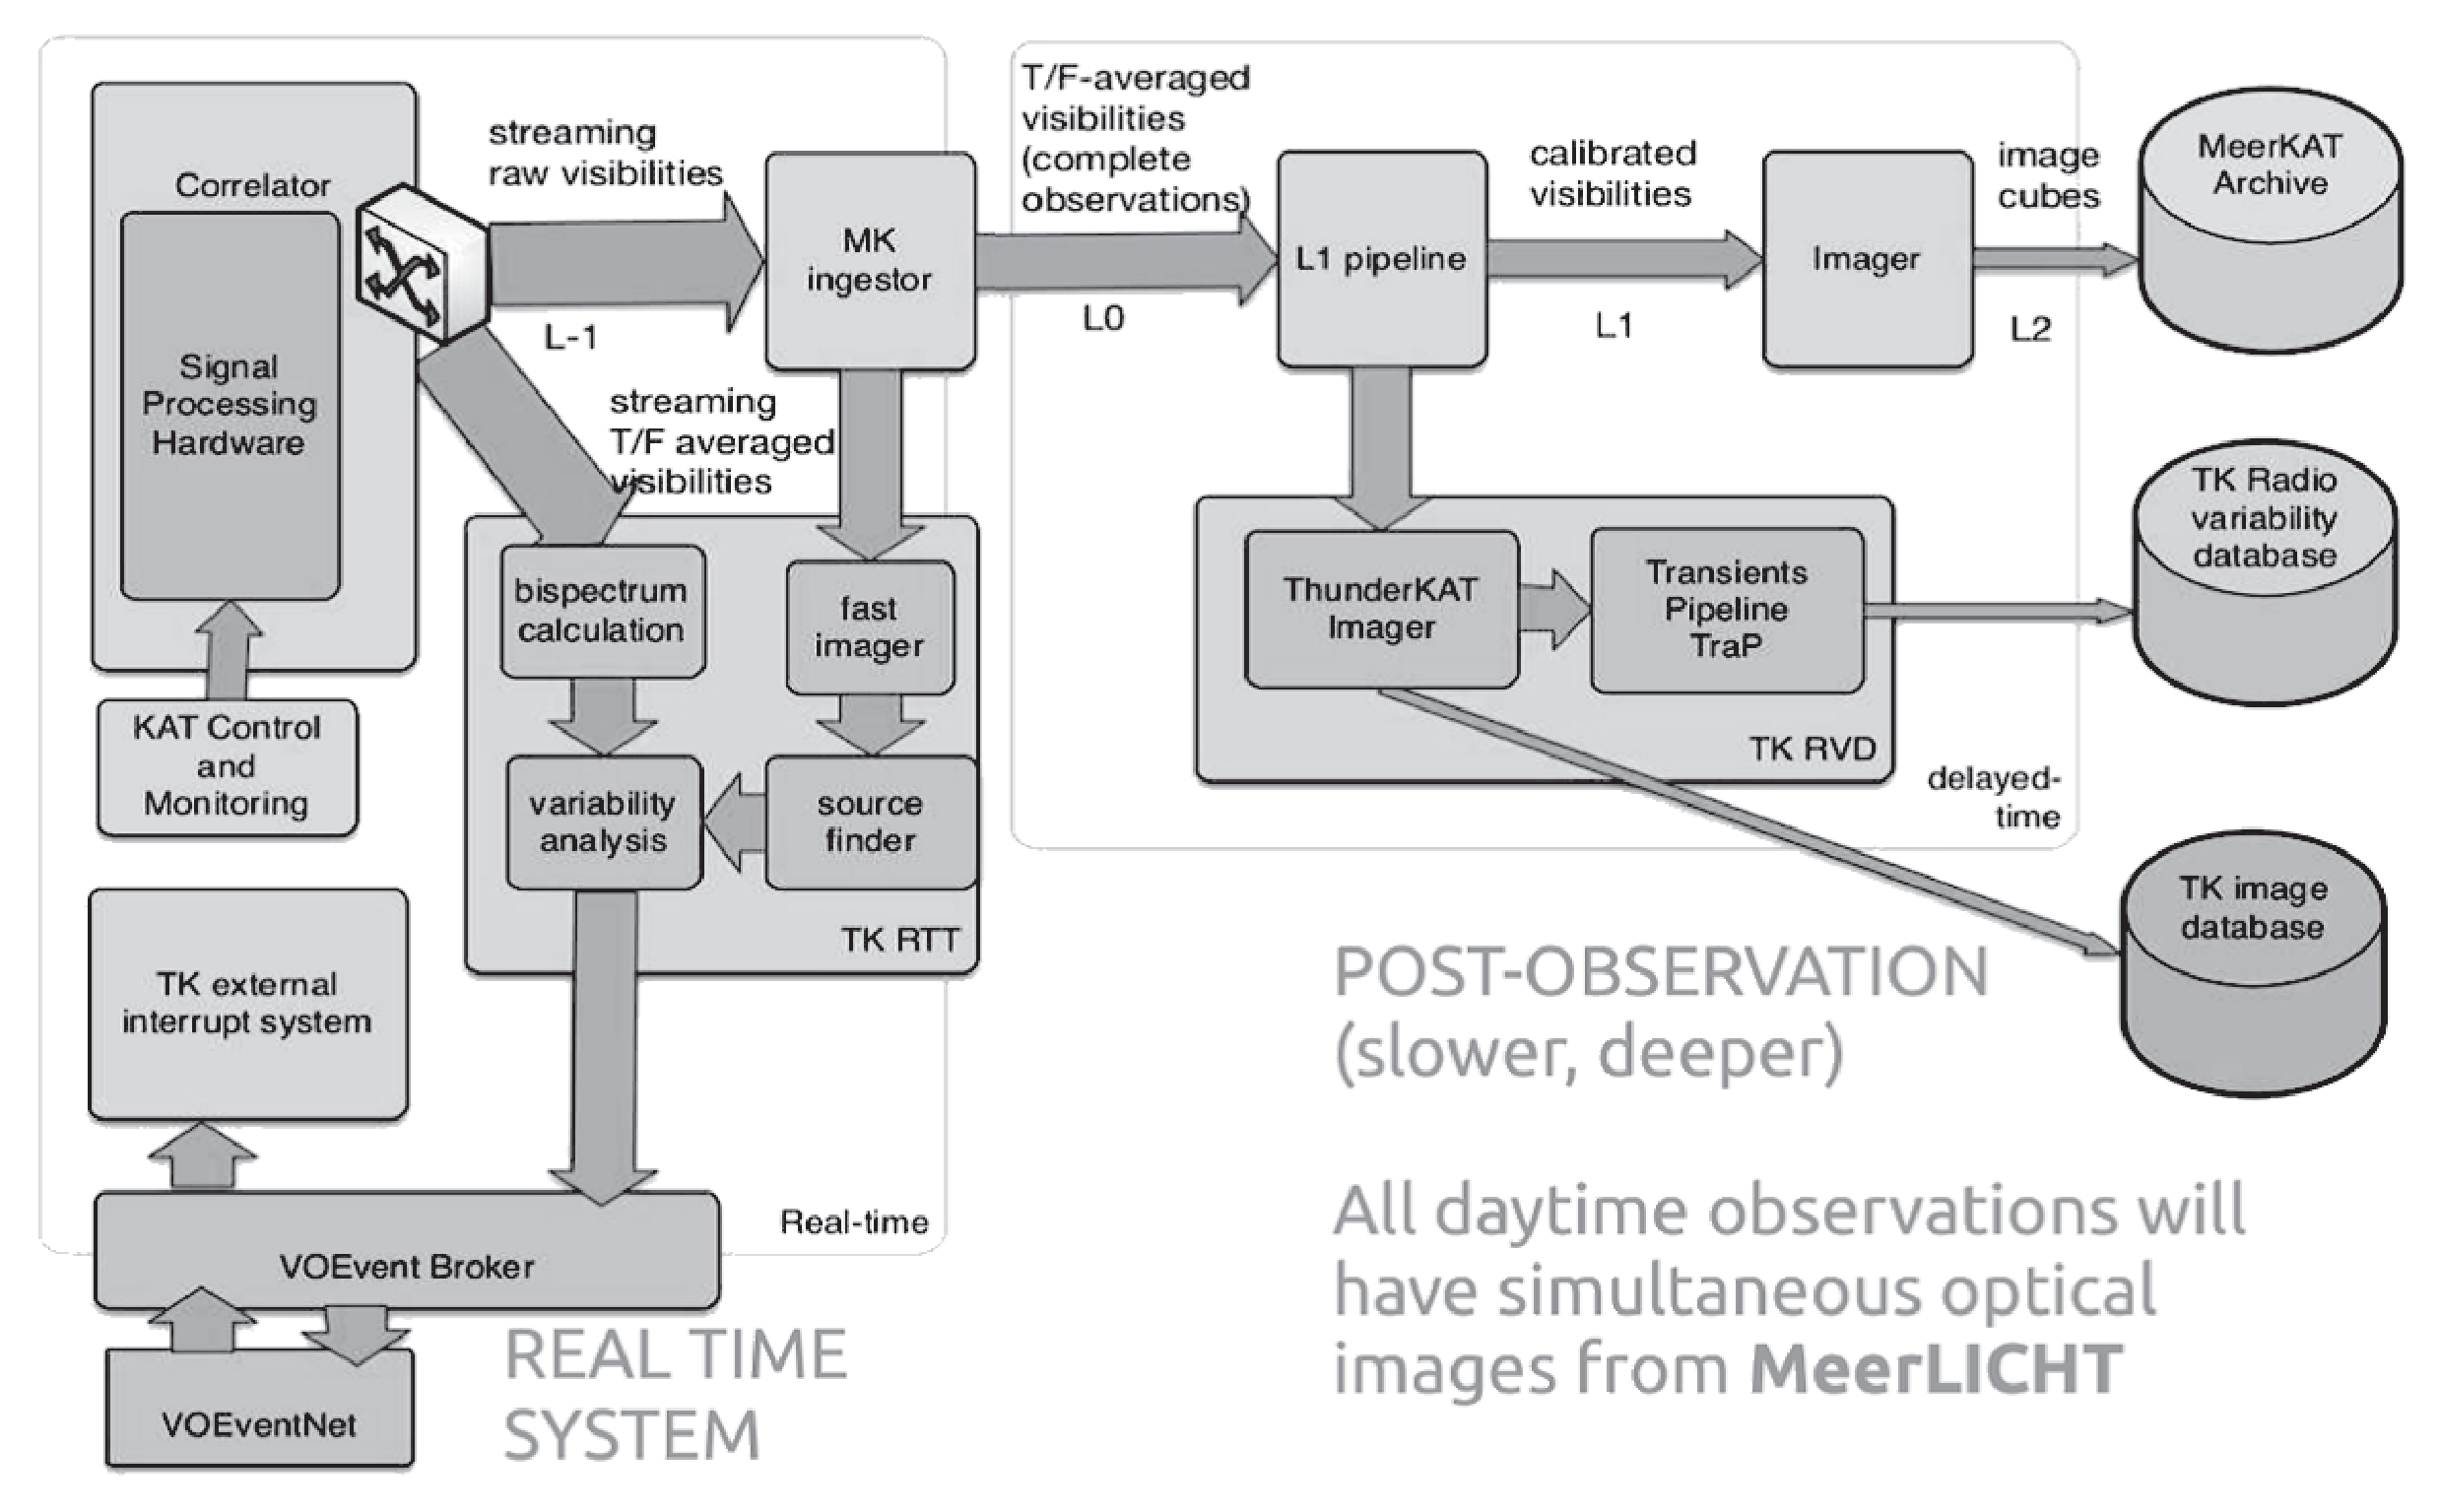
\includegraphics[width=12cm]{transients/transients.s2.fender.commensal.eps}
	\caption{他の観測と共存した突発天体探査システム。}
	\label{fig:transients.fender.commensal}
\end{figure}%

%%
\subsubsection{SKAへの要求 (2): 突発天体発見時の自動的な追観測システム}
%%
突発天体の観測的研究に重要なもう一方のシステムは、他の観測局によって発見された突発天体、あるいはSKA自身によって発見した突発天体を、自動的に追観測するというものである。
このようなシステムは既にイギリスのArcminute Microkelvin Imager Large Array (AMI LA) に実装されており、ガンマ線観測衛星Swiftで発見されたガンマ線バーストを約8時間後に追観測することに成功している \citep{2013MNRAS.428.3114S,2014MNRAS.440.2059A}。
この結果得られた電波帯域での光度曲線から、ガンマ線バーストのリバースショック (星間物質から噴出物の方向に伝わる衝撃波) による電波放射が、世界で初めて確認された。
同様にSwiftの速報によって、地球近傍の連星系 DG~CVn からのガンマ線フレアを6分以内に追観測した結果、電波帯域でも大きいフレアが確認され、広い周波数帯域でのコインシデンスが得られている。
しかし数日後には元の明るさに戻ってしまい、そのようなタイムスケールの短い突発現象を詳細に観測するためには、世界規模で即時的な追観測を行うことが重要である \citep{2015MNRAS.446L..66F}。
SKAにおいても同様のシステムを実装すれば、突発天体の研究にブレイクスルーを起こすことができるだろう。

%%
\subsubsection{まとめ}
%%
突発天体の観測的研究には、SKAに前述の二つのシステムを実装することが重要である。
SKAは広い視野と高い感度を兼ね備えており、さらにそのシステムが実装されれば、電波帯域での変動天体や突発天体を数多く発見することができるだろう。
その発見は、究極の宇宙物理を議論できる場所に、人類を導いてくれるはずである。
突発現象というのは宇宙の、とりわけ深宇宙の灯台であり、その観測によって新しい物理を開拓できるに違いない。


%\setcounter{section}{1}\section{国際SKAサイエンスブックの紹介} \label{c09.s2}

%%%%%%%%%%%%%%%%%%%%%%%%%%%%%%%%%%%%%%%%%%%%%%%
%%%%%%%%%%%%%%%%%%%%%%%%%%%%%%%%%%%%%%%%%%%%%%%
\subsection{ガンマ線バースト}
\label{c09.s2.ss2}

\paragraph{GRB電波残光の観測の現状}

GRBは宇宙で起こる極限現象のひとつであり、基礎的な物理過程を探る自然界の実験場の役を果たすだけではなく、おそらく極限の赤方偏移に至るまでの宇宙の星形成率をトレースし宇宙史に渡る銀河間物質の構成を示すだろう。
GRBの電波観測はGRBの物理特性を決定する中心的な部分を担う。
しかしながら現在までのところ、GRBの電波観測は大抵ガンマ線検出天体のフォローアップ観測に限られてしまっている。

\paragraph{GRB電波残光のSKA観測の見込み}

SKAは、Phase~1 の初期科学段階で高周波帯域で数百の天体をフォローアップし、GRB残光の研究を大幅に進展させるだろう。
\skamid{1}のBand~4 (4~GHz) と Band~5 (9.2~GHz) はとりわけGRB残光のような突発天体現象の探知に向いているだろう。
時間進化する放射スペクトルの光学的厚みの遷移をサンプルしながら、電波残光のピークを探知する。
そして放出物が非相対論的な速さに減速する時間までの残光を追跡できる。
SKA2では全GRBの25\% についてその減速までの残光を観測することができるだろう。
これはGRBの真のエネルギー割当量、周辺の密度分布、そして衝撃波の物理について重要な知見を与えるに違いない。
SKAは、ジェットが地球を向いていないGRBからの orphan afterglow を日常的に探知できるようになるだろう。
\skasur{1} の深い全天サーベイは、毎週300イベント程度のorphan afterglowを検出するだろう。その検出率はSKA2では1000を超えると予想される。

%%%%%%%%%%%%%%%%%%%%%%%%%%%%%%%%%%%%%%%%%%%%%%%
%%%%%%%%%%%%%%%%%%%%%%%%%%%%%%%%%%%%%%%%%%%%%%%
\subsection{太陽質量コンパクト天体からのインコヒーレントな突発的電波放射}
\label{c09.s2.ss3}

\paragraph{太陽質量コンパクト天体と電波放射}

物質降着するコンパクト天体によるジェット形成とアウトフローは、物質降着と物質放出の間の関係によって決まる。
この放出過程におけるインコヒーレントなシンクロトロン放射は、ブラックホール、中性子星、そして白色矮星を含む多くの降着連星天体で観測されている。

\paragraph{電波観測から分かること}

散発的なアウトバースト中の電波放射の進化をモニタリングすることは、ジェットの立ち上がりについて重要な知見を与え、また、より高周波帯での観測と合わせれば、ジェットと降着円盤の潜在的な関係を解き明かすことになるだろう。
電波観測によって、マグネターの巨大フレアなどの爆発的イベントも含めたジェットやアウトフローの、運動学的なフィードバックを定量化することができれば、星周物質への重要性も示すことができる。

\paragraph{感度への期待}

SKAの高感度は、明るいエディントン限界のアウトバースト状態から、元々暗くて詳細な研究ができなかった低光度の鎮静したレベルまで、質量降着する太陽質量コンパクト天体のモニタリングを可能にし、新しいパラメータ空間を切り拓くだろう。
鎮静した質量降着ブラックホールの国勢調査は、連星系の進化過程にも制限を与えるだろう。
これまでのブラックホールジェットの調査を中性子星や白色矮星のより暗いジェットへと拡張することを可能にすることで、SKAはジェット形成におけるコンパクト天体の役割を決めるための比較研究を可能にする。
SKAの高感度と広視野そしてマルチビーム能力を駆使すれば、観測しうる近傍宇宙($\sim$15 Mpc以内)の全ての「明るいフレア天体」の探知とモニタリングが可能となる。
それは初代クェーサーの成長への重要な示唆と共に、質量降着率が極めて高いコンパクト天体におけるジェットの特性について、我々に新たな知見を与えるに違いない。
そこには超高輝度X線源 (ultraluminous X-ray source; ULX) の電波対応も含まれる。

\paragraph{SKA観測の見通し}

シンクロトロン過程は、高周波にて早くピークを迎え、またフラックス密度が大きいので、以上のような研究は\skamid{1}の高周波帯Band~4 と 5 で、最も効率よく観測できるだろう。
\skamid{1} の高い感度があれば、太陽質量ブラックホールや球状星団内の中間質量ブラックホールの存在が想定される領域から、Bondi-Hoyle降着の進む孤立した鎮静ブラックホールを検出することもできるだろう。

%%%%%%%%%%%%%%%%%%%%%%%%%%%%%%%%%%%%%%%%%%%%%%%
%%%%%%%%%%%%%%%%%%%%%%%%%%%%%%%%%%%%%%%%%%%%%%%
\subsection{ジェットを伴う潮汐崩壊現象の強い狩人としてのSKA}
\label{c09.s2.ss4}

\paragraph{潮汐崩壊現象}

超巨大ブラックホール (SMBH) による星の潮汐崩壊現象 (TDE) の観測的な帰結は、鎮静したSMBHを発見することを可能にし、それらの質量関数を制限することにつながる。
それ以上に、かつては活動的ではなかった銀河におけるジェットを伴った潮汐崩壊を観測することは、初期段階、言い換えれば「汚れのない」環境での、ジェット形成と進化を研究するという新しい意味をもたらす。

\paragraph{潮汐崩壊現象の観測}

数から数十の潮汐崩壊は1999年以降発見されてきているが、ジェットを伴った潮汐崩壊はたった2つだけ硬X線によって発見された。そしてそのうちのただ1つ、Swift J1644+57だけが潮汐崩壊現象という解釈をさらに支持するような精密位置決定がなされた。これら2イベントだけでは上記の科学的問題に取り組むには不十分であり、サンプルをもっと圧倒的に増やさなければ取り組めない。

\paragraph{SKAへの見通し}

X線は実際に観測された電磁波帯にも関わらず、現在または近い将来のX線装置はジェットを伴った潮汐崩壊現象を発見する最有力装置とはならないだろう。
それらはせいぜい年間で数から数10のイベントを与えるのみと考えられる。
実際の所、潮汐崩壊現象を検出し多波長フォローアップのトリガーをかけるためのベストな戦略は、SKAを用いることである。
SKAは年間で数100のイベント、赤方偏移で$z\simeq 2$程度までのイベントを発見できるだろう。
とはいえ、電波とX線のシナジーは原理的に、ジェットを伴った潮汐崩壊現象の絶対的な発生率、それらのジェットのパワー、群ローレンツ因子、ブラックホール質量関数、といった重要な物理量を制限することができる。
そしておそらく、質量が$10^5~\text{M}_\odot$以下の中間質量ブラックホールを見つけることができるだろう。
最終的に、Large Synoptic Survey Telescope (LSST) などの可視光サーベイとSKAを比べることで、ジェット発生効率をより直接的に制限することができる。

%%%%%%%%%%%%%%%%%%%%%%%%%%%%%%%%%%%%%%%%%%%%%%%
%%%%%%%%%%%%%%%%%%%%%%%%%%%%%%%%%%%%%%%%%%%%%%%
\subsection{宇宙論的距離の早い突発現象}
\label{c09.s2.ss5}

\paragraph{早い突発現象の活用}

宇宙論的距離にわたって探知しうる電波バーストは、銀河間物質 (IGM) と銀河間磁場、そして時空そのものの強い証拠の一つとなる。
それらの分散測度 (DM) は、いわゆる近傍赤方偏移宇宙の「ミッシングバリオン」を解く鍵となり、銀河形成・フィードバックモデルのキーパラメータである銀河ハロープロファイルの初測定を可能にするだろう。
電波バーストは赤方偏移$z\simeq 2$を超えるところでの宇宙のものさしとして使うことができ、ダークエネルギーの状態方程式のパラメータ$w(z)$を、Ia型超新星で測られている赤方偏移をはるかに超えて制限することができる。
これらの科学成果は、可視光フォローアップでホスト銀河の赤方偏移を得るのに十分な1\arcsec 以内に位置精度が収まる、およそ$10^4$のFRBサンプルによって実現できる。
重力波イベントはSKA1-LOW帯域でコヒーレントな放射をすると仮定すると、宇宙論的な距離のFRBの位置決定は宇宙論的な標準サイレンとして使うことができる。

\paragraph{SKAへの見込み}

以上のような研究を実施するためには、発見したFRBのDM, RM, SMと比べられるように、FRBのホスト銀河を特定し、その赤方偏移を測定しなければならない。
そしてこれは、半径3~km 内に全アンテナの80\% を集めたコンパクト構成による集光デザインで実現でき、また高時間分解の信号処理機器を伝送路上に設置することが求められる。

%%%%%%%%%%%%%%%%%%%%%%%%%%%%%%%%%%%%%%%%%%%%%%%
%%%%%%%%%%%%%%%%%%%%%%%%%%%%%%%%%%%%%%%%%%%%%%%
\subsection{ガンマ線バーストを用いた宇宙論へのSKAの貢献}
\label{c09.s2.ss6}

\paragraph{GRB宇宙論}

ガンマ線バースト (GRB) の光度は一定ではなく標準光源ではないが、宇宙の幾何学と膨張率を測るツールとして注目されている。
それはFRBの$10^{53}~\text{erg/s}$を超える膨大な光度と、$z=8$を超える高赤方偏移というユニークな組み合わせによる。
近年、GRBを標準化し宇宙論パラメータ推定に使うために、いわゆる$\nu F_\nu$スペクトルのピーク光子エネルギーと、放射の強度 (放射されたエネルギーないし光度) の関係を活用するいくつかの試みがなされた。
これらの研究によって、既存のGRBデータから$\Lambda$CDM宇宙模型の物質パラメータ$\Omega_\text{M}\sim 0.3$が導き出された。
現在そして次世代のGRB観測 (Swift, Fermi, SVOM, UFFO)\footnote{SVOM: Space Variable Objects Monitor; UFFO: Ultra-Fast Flash Observatory.} により期待される結果から、ダークエネルギーの特性と進化の手がかりをつかむことが可能となるだろう。

\paragraph{SKAへの見込み}

SKAを用いたGRBの電波観測および他波長観測の結果から、従来は得られなかったGRBの特徴が明らかとなるだろう。
GRBの研究はSKAのその他の天体に関する主要科学計画の観測を補い、SKAの主要科学目的のいつくかに重要な貢献をすると期待できる。

%%%%%%%%%%%%%%%%%%%%%%%%%%%%%%%%%%%%%%%%%%%%%%%
%%%%%%%%%%%%%%%%%%%%%%%%%%%%%%%%%%%%%%%%%%%%%%%
\subsection{活動銀河核の時間領域研究}
\label{c09.s2.ss7}

\paragraph{AGNの時間領域研究の背景}

活動銀河核 (active galactic nucleus; AGN) の電波変動の観測は、内在的な変動と外来的な変動の両方を明らかにすることができる。
内在的なものは衝撃波・フレア・超巨大ブラックホール周りの放射の変化、外来的なものはたとえば天の川銀河の構造による散乱が原因である。
そのような星間散乱はマイクロ秒角の空間分解能で放射領域の構造を示す。
現在までのAGN観測は、長期間モニターされ続けた天体が少ない、あるいは、モニター数は多いが時間分解能に乏しい、といういずれかの問題を抱えていた。

\paragraph{SKAへの見込み}

SKAを用いることによるサーベイ能力の劇的な向上は、毎日かそれ以下の頻度で10万個のAGNの精密な外観モニター研究を可能にする。
変動の統計、特に多周波同時観測は、AGNのクラス、光度、そしてジェット指向性という多くの問題を解決し、質量降着の物理を示すだろう。
また星間物質による電波散乱の原因となる構造を、詳細に解明できるだろう。

%%%%%%%%%%%%%%%%%%%%%%%%%%%%%%%%%%%%%%%%%%%%%%%
%%%%%%%%%%%%%%%%%%%%%%%%%%%%%%%%%%%%%%%%%%%%%%%
\subsection{コア崩壊型超新星とIa型超新星}
\label{c09.s2.ss8}

\paragraph{コア崩壊超新星}

コア崩壊型超新星 (core-collapse supernova; CCSN) からの電波放射の系統的な調査はいまだなく、狙いをつけた調査、つまり近傍宇宙のいくつかの可視光で発見されたCCSNからの電波のみが観測されてきた。
可視光での調査はダスト減光により大部分のCCSNを見損なう。
ゆえにCCSNの電波での調査は覆い隠されていない完全な近傍宇宙の星形成率を与えることに有望である。
SKAはこの領域の調査に、他の目的の観測に「相乗り」する形で、広視野のブラインドサーベイを行うことが重要である。
計画中の VLA Sky Survey (VLASS) が最大でも数10個のCCSNを発見する見込みに対して、\skasur{1}はたった1年で数100個のCCSNを発見し、SKA1の10倍の感度を持つSKA2では近傍宇宙で数千個のCCSNを探知すると期待される。
ゆえに相乗り観測モードは、近傍宇宙におけるほぼ全てのCCSNの国勢調査を簡単になしうる。
ゆえにCCSNの体積発生率 (イベントレート) を正確に決定するだろう。

\paragraph{Ia型超新星}

Target of Opportunity (ToO) 観測の運用体制を確立し、近傍 ($\lesssim 25~\text{Mpc}$) のIa型超新星を爆発から数日以内に追観測できるようにすることを提言する。
SKAの比類なき感度は、爆発シナリオがsingle-degenerateなのかdouble-degenerateなのかを曖昧なく区別することを可能にするだろう。

%%%%%%%%%%%%%%%%%%%%%%%%%%%%%%%%%%%%%%%%%%%%%%%
%%%%%%%%%%%%%%%%%%%%%%%%%%%%%%%%%%%%%%%%%%%%%%%
\subsection{新星と共生連星からの熱電波放射}
\label{c09.s2.ss9}

\paragraph{星系からの突発現象}

熱的な電波放射は星系からのアウトフローの本質的なトレーサーである。
新星と共生連星\footnote{共生連星または共生星とは、主星が伴星である赤色巨星の中に入り込んでしまった連星系である。}は白色矮星上の質量降着と核燃焼を内包した相互作用する連星系である。
それらからのアウトバーストのほとんどは、高周波帯でより高いフラックス密度をもち、時間的に変動し、そして銀河面に大体集まっている、という特徴をもつ。
自由--自由放射による物理的描像は、シンクロトロン放射による描像とは独立していて相補的である。
SKAの潜在能力を駆使し、熱的過程の高精度な観測を行うことが重要である。

\paragraph{新星の観測}

アウトバースト時の新星の熱的電波放射は放出質量、運動エネルギー、そして放出物の密度分布といったプロファイルを反映し、その観測によっておそれらを解明することができる。
VLAやe-MERLINなどによる最近の観測では、新星の質量放出の信じられないような複雑な過程、例えば放出過程に多くの段階があることや、時間的に長期に渡って起きているように見える、というような問題を解き明かし始めている。

\paragraph{共生連星の観測}

共生連星もアウトバーストを示す。
それはときどきジェットの物質排斥に伴なわれる。
しかしながら、新星と違って共生連星の長期間の熱放射は、熱い白色矮星に照らされた巨大伴星の風の中に由来する。
巨星風における白色矮星の影響は時間的に変動し、そしてそれらの変動を駆動する物理過程は謎のままである。
おそらく質量降着の不安定性や白色矮星表面での時間変動する核燃焼によるものと考えられている。

\paragraph{SKAへの期待}

SKA1の感度は天の川銀河全域に渡って新星サーベイをすることを可能にするだろう、そしてそれにより統計的に完全な分布が暴かれる。
SKA2をもってすれば、同様のことをマゼラン銀河でもできるようになるだろう。
これはIa型超新星の発生源としてそれらの可能な役割を決定するための重要な示唆とともに、白色矮星への質量降着と質量欠損の背後の理論について、質の高いテストを可能にする。
\skamid{1}の特に高周波を優先した広帯域観測によって、新星の多様性を招いている物理過程について多角的な考察が可能となり、共生連星の質量降着過程と降着率を導き出すだろう。

%%%%%%%%%%%%%%%%%%%%%%%%%%%%%%%%%%%%%%%%%%%%%%%
%%%%%%%%%%%%%%%%%%%%%%%%%%%%%%%%%%%%%%%%%%%%%%%
\subsection{超新星と超新星残骸の研究}
\label{c09.s2.ss10}

\paragraph{超新星の種類}

超新星は究極的に明るく、そして数日間は銀河全体よりも明るくなりうる。
その爆発のシナリオとして主に2つのものが考えられており、白色矮星の熱核反応爆発 (Ia型) と大質量星のコア崩壊 (II型、Ib型、Ic型) である。

\paragraph{Ia型からの電波を捉える}

Ia型超新星爆発は宇宙の加速膨張を発見するための遠方の指標、標準光源として用いられてきた。
しかしそれらの発生源系はいまだに困惑の種である。
爆発による前方衝撃波とその周りの星周物質 (circumstellar matter; CSM) ないし星間物質 (Interstellar medium; ISM) の間の相互作用による電波放射は、超新星爆発の最後の進化局面を見るための重要なプローブである。
しかし、現在の電波望遠鏡によってIa型の爆発そのものからの電波放射は検出されていない。
SKAは高い感度と分解能によって、このIa型超新星爆発の電波を初探知できるかもしれない。

\paragraph{可視光で見えないII型を見つける}

II型超新星には、可視光で暗いものは元々暗いかダストの減光によって見そこねているという「超新星爆発頻度問題」というものがある。
多くのダストに包み隠されて可視光で見えない超新星爆発が\skamid{1}や\skasur{1}で見つけられるだろう。
特にホスト銀河の最内部に位置するものが見えてくると期待される。
さらに、元々暗いものの発見もSKA1でもたらされるだろう。
また探査で明らかとなるイベントレートによって、現在の星形成率と初期質量関数にあらたな情報をもたらすに違いない。

\paragraph{超新星残骸のSKA観測}

超新星爆発は周囲のCSMやISMを吹き飛ばしながら、過熱する衝撃波を引き起こし、そして超新星残骸 (SNR) を作り出す。
そしてより多くのSNRがSKAによって発見されると期待される。
これは現在問題となっている、超新星の理論的予測と観測との間のずれを減らすだろう。
複数のSNRは宇宙線の主たる成分である陽子を、その衝撃波で高エネルギーにまで加速していると確認されている。
SKAと Cherenkov Telescope Array (CTA) の観測を組み合わせることで、銀河宇宙線の起源のパズルを解く希望をもたらすだろう。


%%%%%%%%%%%%%%%%%%%%%%%%%%%%%%%%%%%%%%%%%%%%%%%
%%%%%%%%%%%%%%%%%%%%%%%%%%%%%%%%%%%%%%%%%%%%%%%
\subsection{系内外のブラックホールX線トランジェントの早期検出と網羅}
\label{c09.s2.ss12}

\paragraph{SKAへの期待}

SKAの低周波における広視野と高感度によって、超巨大ブラックホール近傍での潮汐崩壊現象 (TDE) や太陽質量ブラックホール (low-mass X-ray binary; LMXB) でのフレア、またアウトバーストの進む系内外の突発天体を数多く発見できるであろう。
将来のX線広視野モニター観測と比較しても、SKAこそが最初にイベントを発見しアラートを他の観測所に送信することができる。
一方で、TDEフレアや突発的アウトバーストの立ち上がり期の質量降着率は幅広く変化するので、SKAは広範囲に渡る質量降着率とその変化率を網羅することができる。
そしてそれらの量は、定常的に電波を放射するブラックホール系においては、観測不可能なパラメータ空間である。
非定常な降着状態にあるブラックホール近傍からの突発現象を観測することで、降着円盤とジェットの関係に関する我々の理解を研ぎ澄ませるだろう。


\subsection{未知の未知} \label{transients.s2.wilkinson}
アメリカ合衆国国防長官だったラムズフェルド氏の言葉 \citep{Rumsfeld} を借りると、物事には三種類あり、それらは
\begin{description}
	\setlength{\leftskip}{1cm}
	\item[Known knowns:] 我々が既に知っている事実、
	\item[Known unknowns:] 我々が知らないことを自覚している未知、
	\item[Unknown unknowns:] 我々が知らないことを自覚すらしていない未知、
\end{description}
というものである。
このことは、宇宙科学の分野においてもまったく同様である。
そこで本節では、unknown unknowns つまり未知の未知に相当する、予想すらできていない未知の天体現象の探査 (exploration of unknowns; EoU) について述べる。
とりわけ未知を発見するために持っておくべき哲学と、その哲学に基づいたSKAへの要求仕様を紹介する。

%%
\subsubsection{未知追究の哲学}
%%
宇宙科学における known knowns は既に研究されてきていることであるから、もしそれについて知りたければ文献を読めばよい。
一方 known unknowns について知りたければ、何を知るべきか把握していることなので、観測提案書を書いて観測を実施すればよい。
その観測が成功すれば、known unknowns は known knowns に変わり、宇宙科学は一歩前進することになるだろう。
しかしながら unknown unknowns については、我々はその存在にすら気付いておらず「知らないということすら知らない」。
そのため、どんな研究をしてどんな観測をすれば良いのか、検討するどころか見当すらつかない。
しかし過去の偉大な科学的発見が、そのような unknown unknowns を偶然発見したことに端を発しているのも事実である。

ゆえにSKAが長期に渡って科学成果を出し続けるためには、そのような unknown unknowns を発見できる能力を備えておかなくてはならない。
SKAは、前章までに述べてきたような「現在」未解決とされている問題に対して注力し、その解決を目標とする。
%それらの問題の解決は非常に重要であり、その実現によって宇宙科学は大きく前進することだろう。
しかしSKAが完成し隆盛を誇っているだろう2025年以降には、現在未解決のそれらの問題は既に解決されているに違いない。
その時SKAによる興奮はどこにあるかと言えば、それは解決済みの古い問題にはなく、新しい観測方式によって浮上するだろう新しい疑問、つまり unknown unknowns にある。
%人間はこの宇宙や構成物を第一原理から創り出せるほど、創造力も想像力もない。
それゆえ天文学では、我々が想像すらしていない「未知の何か」を見つけるための「備え」が重要であり、その備えに裏打ちされた「発見」が重要となる。

%%
\subsubsection{未知の探査 (EoU) のための要求}
%%
電波天文学における unknown unknowns がどのような天体現象なのかはもちろん予測できないが、「起源のわからない未知の突発現象」が既に発見されてきている。
%前述のとおり電波帯域における突発現象の中には、それを放射した実体がどのような天体なのか、あるいはどのような放射機構によって突発的な電波放射がなされたのか、わかっていないものが少なくない。
%第~\ref{transients.s1}節で述べたとおり、電波帯域における突発現象の中にはそれを放射した実体や放射機構がわかっていないものが多い。
%そのような未知の突発現象は、MHz から GHz という低周波帯域で、集光面積の大きな望遠鏡によって発見されていることが多い。
しかしそれらを発見した望遠鏡は、そのような未知の現象を捉えようとして設計されたわけではなかったし、何らかの理論をもとにして突発天体を探査したわけでもなかった。
ところが蓋を開けてみれば、未知の突発現象が次々と発見され、新たな科学が生まれている。
そしてこれからも、まだ予想もされていないような変動現象や突発現象が次々に見つかるに違いない。
それを効率的に発見できるのが、SKAである。

SKAは高い感度と広い視野を持っており、未知の現象を数多く発見できる潜在能力がある。
ただし潜在能力があったとしても、それを有効に活用できなければ未知の探査は進まないだろう。
SKAがその潜在能力を解放し未知の探査を効率的に行うためには、第~\ref{transients.s1}節で述べたような (1) 共存システムや (2) 自動追観測システムを活用できるような「柔軟性」が必要である。
%SKAがその潜在能力を解放し未知の探査を効率的に行うためには、次のようなシステムの柔軟性と拡張性が必要となる:
%\begin{itemize}
%	\item 小規模な試験観測を可能にすること、
%	\item 他の観測と共存・並行して突発天体を探査できるようにすること、
%	\item 突発天体の発見速報を受けた際に、すばやく観測モードを変更して追観測を行うこと。
%\end{itemize}
%SKAを長期間運用することを考えると、しばしば技術的な試験を行う必要性が出てくると思われる。
%そのときに例えば、一つあるいは複数のアンテナを用いて小規模な試験観測をできるような柔軟性があると、その後の観測が向上するだろう。
%また突発現象観測では第~\ref{transients.s2.fender}節で述べたように、ある観測と並行して別の観測も行えるような拡張性高いシステムと、緊急時に観測モードをすばやく再設定できるような柔軟性も必要である。
またそのようなシステム柔軟性の他に、観測後のデータ解析においては次の二つの要素が重要となる。

%\paragraph{要素 1: 一般市民による科学}
\paragraph{要求 1: Einstein@Home と同様のプロジェクト}
SKAを有効活用するには、その観測データが研究者だけでなく一般人にも開かれていることが重要である。
多くの人にSKAデータを解析してもらい、彼らの興味を最大限に引き出せるような環境を用意しなければならない。
この「一般市民による科学」には既に前例があり、重力波望遠鏡 LIGO や Arecibo 天文台の観測データを一般市民のコンピュータで解析してもらうプロジェクト、Einstein@Home\footnote{Einstein@Home: \url{http://www.einsteinathome.org/}} によって新しいパルサーが数多く発見されてきている。
同様のプロジェクトを SKA でも行うことで、SKAによる成果を最大化できるのみならず、人類全体による科学探求が実現するだろう。

%\paragraph{要素 2: 他の望遠鏡とのシナジー}
\paragraph{要求 2: Virtual Observatory への貢献}
SKAを有効に活用するには、前述の一般市民による科学と併せて「他の望遠鏡とのシナジー」を最大化することも重要である。
第~\ref{transients.s1}節で述べた (2) 自動追観測システムもそのシナジーのひとつであり、天体を連携して観測し多くの情報を得ることで、高いシナジー効果が生まれるだろう。
これは観測の最中に期待できるシナジーだが、観測が終わりデータだけが残っている状態でも、他の望遠鏡とのシナジーを図ることができる。
それを実現するのが Virtual Observatory\footnote{Virtual Observatory (VO; \url{http://www.ivoa.net/}) は観測データをデータベース化したり、扱いやすいデータ解析ツールを提供しているプロジェクトである。日本でも JVO (\url{http://jvo.nao.ac.jp/}) が活動し、一般市民もすばる望遠鏡などのデータにアクセスしやすくなっている。} (VO) であり、VO を利用することによって、複数の望遠鏡による多波長観測データを容易に比較できる。
したがって他の望遠鏡とのシナジーを飛躍的に高めるために、SKAはそのデータリソースをVOにつぎこむことが重要であり、それによって多くの科学成果を生むことができるだろう。


%%
\subsubsection{まとめ}
%%
%宇宙の現象のほとんどは既存の望遠鏡によって調べつくされている、と考える人もいるかもしれない。
%しかし実際にはそのようなことはない。
%なぜなら、それを調べようとして調べたものしか調べられていないからである。
%我々がまだ想像もしていないような未知の現象 (unknown unknowns) が宇宙にはあふれていると思われ、図~\ref{fig:transients.phasespace}の空白領域がその事を示唆している。
宇宙には、我々がまだ想像すらしていないような未知の現象 (unknown unknowns) があふれていると考えられ、図~\ref{fig:transients.phasespace}の空白領域がその事を示唆している。
アメリカの作家であり生化学者でもあるアイザック・アシモフが言ったとされている言葉に次のようなものがある。
\begin{quote}
%The most exciting phrase to hear in science, the one that heralds new discovery, is not ``Eureka!'' but ``That's funny...''\\
---科学において最も興奮する言葉、つまり新しい発見の前兆となる言葉は、「わかった!」ではなく「これは妙だな...」である。
\end{quote}
つまり known unknowns を解明したときの「わかった」という言葉よりも、unknown unknowns を発見したときの「妙だな」という言葉の方が、科学にとっては面白いということである。
SKAは、そのような未知の発見に備えて設計されなければならず、そのためには第~\ref{transients.s2.fender}節で述べたような柔軟な観測システムが不可欠である。
また、未知の発見に「備えておく」ことの重要性は、フランスの生化学者であるルイ・パスツールの言葉にも見ることができる。
\begin{quote}
%In the fields of observation chance favors only the prepared mind.\\
---チャンスはそれに備えている者だけにほほえむ。
\end{quote}
つまり、科学にとって最も面白い「これは妙だ」と言える未知を発見するには、その発見のチャンスが舞い降りることに備えておかなければならない。
その「備え」として、SKAには観測システムの「柔軟性」が不可欠である。
それとともに、一般市民が探査に参加できるようにすることや、他の望遠鏡とのシナジー効果を最大化することも重要となる。
それらを実現することで、SKAは長期にわたって科学成果を出し続けることができる。
